\subsection{Formale Begriffsanalyse}
Die \ac{FBA} ist ein mathematischer Formalismus, welcher es ermöglicht gegebene Daten auf hierarchische relationale Zusammenhänge zu analysieren \cite{formale-begriffsanalyse, formal-concept-analysis-wille}.
Ein formaler Kontext ist ein Tripel $\mathbb{K} \coloneqq (G, M, I)$, wobei $G$ die Menge der Gegenstände, $M$ die Menge der Merkmale und die Menge der Inzidenzrelationen $I \subseteq G \times M$ definiert.
Gegenstände können als Kategorisierung von Daten verstanden werden, während Merkmale die Eigenschaften der Gegenstände beschreiben.
Eine Inzidenzrelation ist eine binäre Relation, welche angibt, ob ein Gegenstand ein Merkmal aufweist.
Sie besteht aus Tupeln der Form $(g,m)$ mit $g \in G$ und $m \in M$.
Ein formaler Begriff des Kontextes $\mathbb{K}$ ist ein Tupel $(A,B)$, wobei $A \subseteq G$ und $B \subseteq M$.
Die Ableitung von $A$ ist definiert als $A' \coloneqq \{m \in M \mid \forall g \in A, (g,m) \in I\}$.
$A'$ ist der Inhalt (Extent) von $A$.
Analog kann für Teilmenge $B$ der Umfang (Intent) $B'$ bestimmt werden mit $B' \coloneqq \{g \in G \mid \forall m \in B, (g,m) \in I\}$.
Für einen formalen Begriff gilt, dass $A = B'$ und $B = A'$.\\

\begin{center}
    \begin{table}[!ht]
        \centering
        \resizebox{\textwidth}{!}{
            \begin{tabular}{|l||c|c|c|c|}
                \hline
                                  & Nahrungsmittel & Pflanzliche Nahrungsmittel & Tierische Nahrungsmittel & Getreide \\ \hline \hline
                Apfel             & $\times$       & $\times$                   &                          &          \\ \hline
                Rindfleisch       & $\times$       &                            & $\times$                 &          \\ \hline
                Weizen            & $\times$       & $\times$                   &                          & $\times$ \\ \hline
                Hafer             & $\times$       & $\times$                   &                          & $\times$ \\ \hline
                Rindfleischburger & $\times$       & $\times$                   & $\times$                 & $\times$ \\ \hline
            \end{tabular}
        }
        \caption{Kreuztabelle - Nahrungsmittel}
        \label{table:fca-food}
    \end{table}
\end{center}

% Tabelle & Implikation
\autoref{table:fca-food} zeigt beispielhaft die Visualisierung eines formalen Kontextes $\mathbb{K}$ in Form einer Kreuztabelle.
In dieser Tabelle sind die Gegenstände als Zeilen und die Merkmale als Spalten beschriftet.
Ein Kreuz $\times$ gibt an, ob ein Gegenstand ein Merkmal aufweist.
Also, ob ein Tupel der Form $(g,m)$ in der Menge der Inzidenzrelationen $I$ enthalten liegt.
Der Gegenstand Weizen besitzt drei Inzidenzrelationen.
Er steht jeweils mit den Merkmalen Nahrungsmittel, pflanzliche Nahrungsmittel und Getreide in Relation.
Betrachtet man die Kreuztabelle näher, so fällt auf, dass alle Gegenstände, welche das Merkmal Getreide aufweisen, auch das Merkmal pflanzliche Nahrungsmittel aufweisen.
Dies ist ein Beispiel für eine Implikation zwischen Merkmalen.
Dabei gilt für zwei Mengen von Merkmalen $M_1, M_2 \subseteq M$, dass $M_1\implies M_2 \coloneqq M_1' \subseteq M_2'$.\\

% Beispiel & A'' = A
Für ein besseres Verständnis der \ac{FBA} werden weitere Beispiele anhand der \autoref{table:fca-food} erläutert.
Ein formaler Begriff des Kontextes $\mathbb{K}$ ist das Tupel $(A_1, B_1)$ mit:
\begin{align}
    A_1 & = \{Weizen, Hafer, Rindfleischburger\} \subseteq G                     \\
    B_1 & = \{Nahrungsmittel, Pflanzliche\ Nahrungsmittel,Getreide\} \subseteq M
\end{align}
Für den Inhalt von $A_1'$ und dem Umfang von $B_1'$ gilt:
\begin{align}
    A_1' & = \{Nahrungsmittel, Pflanzliche\ Nahrungsmittel, Getreide\} \\
    B_1' & = \{Weizen, Hafer, Rindfleischburger\}
\end{align}
Somit gilt die vorher erwähnte Definition für den formalen Begriff $A_1 = B_1'$ und $B_1 = A_1'$.
Ebenfalls lässt sich durch die Ableitungen im Beispiel eine weitere Eigenschaft von Ableitungen erkennen.
Für die Ableitung von $A'$ gilt $A'' = A$ und für $B$ gilt $B'' = B$.
Dies gilt jedoch nur für einen formalen Begriff.
Verdeutlichen lässt sich durch ein weiteres Beispiel:
\setcounter{equation}{0}
\begin{align}
    A_2   & = \{Weizen\}                                                \\
    A_2'  & = \{Nahrungsmittel, Pflanzliche\ Nahrungsmittel, Getreide\} \\
    A_2'' & = \{Weizen, Hafer, Rindfleischburger\}
\end{align}
Für eine beliebige Teilmenge $A \subseteq G$ gilt $A \subseteq A''$ und für $B \subseteq M$ gilt $B \subseteq B''$.
Der Grund dafür, dass $A'' = A$ und $B'' = B$ nur für einen formalen Begriff gilt, ist, dass ein formaler Begriff die größtmöglichen Mengen darstellt, welche durch Ableitungen von $A$ und $B$ erzeugt werden können.

\begin{figure}[!ht]
    \centering
    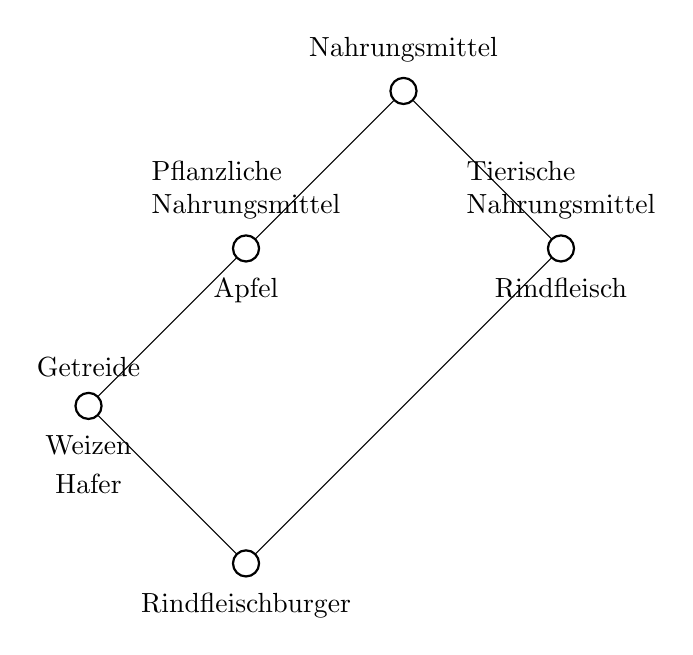
\begin{tikzpicture}
        \begin{scope}[every node/.style={circle,thick,draw}]
            \node (A) at (4,6) {};
            \node (B) at (2,4) {};
            \node (C) at (6,4) {};
            \node (D) at (0,2) {};
            \node (E) at (2,0) {};
        \end{scope}

        % Merkmale
        \draw (A) +(0,0.25) node[above] {Nahrungsmittel};
        \draw (B) +(0,0.25) node[above, align=left] {Pflanzliche\\ Nahrungsmittel};
        \draw (C) +(0,0.25) node[above, align=left] {Tierische\\ Nahrungsmittel};
        \draw (D) +(0,0.25) node[above] {Getreide};

        % Gegenstände
        \draw (B) +(0,-0.25) node[below] {Apfel};
        \draw (C) +(0,-0.25) node[below] {Rindfleisch};
        \draw (D) +(0,-0.25) node[below] {Weizen};
        \draw (D) +(0,-0.75) node[below] {Hafer};
        \draw (E) +(0,-0.25) node[below] {Rindfleischburger};

        % Relationen
        \draw (A) -- (B);
        \draw (A) -- (C);
        \draw (B) -- (D);
        \draw (C) -- (E);
        \draw (D) -- (E);
    \end{tikzpicture}
    \caption{\label{fig:begriffsverband}Begriffsverband - Nahrungsmittel}
\end{figure}

% Begriffsverband
Die Daten von \autoref{table:fca-food} können als Begriffsverband visualisiert werden.
Dabei werden die gegebenen Daten als Liniendiagramm, wie in \autoref{fig:begriffsverband}, dargestellt. % TODO: cite? \cite{introduction-lattices}
Im Liniendiagramm repräsentieren Knoten Relationen zwischen Merkmalen und Gegenständen.
Über einem Knoten sind die Merkmale und unter einem Knoten die Gegenstände aufgeführt.
Die Verbindung zwischen den Knoten repräsentiert die Implikationen von Merkmalen.
Die Knoten werden dabei in Verbindung zu anderen Knoten gemäß der Regeln einer Ordnung gesetzt.
Für diese gilt, dass die Knoten die folgenden Eigenschaften besitzen:
\begin{align}
    x \leq x \tag{reflexiv}                                       \\
    x \leq y \land y \leq x \Rightarrow x=y \tag{antisymmetrisch} \\
    x \leq y \land y \leq z \Rightarrow x\leq z \tag{transitiv}
\end{align}

Zwischen den Knoten bestehen im Begriffsverband hierarchische Beziehungen.
Das bedeutet, dass der Knoten $x$ unterhalb des Knotens $y$ liegt, wenn $x \leq y$ gilt.
Dabei lassen sich grundsätzlich zwei Leserichtungen für das Liniendiagramm definieren.
Die erste Leserichtung geht von unten nach oben und beschreibt einen Gegenstand $g$ durch die Merkmale $m$, die erreicht werden können, wenn man den Linien im Diagramm nach oben folgt.
Durch die zweite Leserichtung werden alle Gegenstände $g$ eines Merkmals $m$ aufgelistet, welche durch das Verfolgen der Linien im Diagramm von oben nach unten erreicht werden können.
Sowohl die erste als auch die zweite Leserichtung können Knoten enthalten, welche nach oben oder unten mehrere Linien aufweisen.
In diesem Fall werden alle Pfade verfolgt.
Die erste und zweite Leserichtung ist dabei nichts anderes als Inhalt und Umfang für Gegenstand und Merkmal eines Knotens. \\

Im Begriffsverband aus \autoref{fig:begriffsverband} ist der Gegenstand Apfel unter dem Merkmal pflanzliche Nahrungsmittel zu finden.
Um den Inhalt dieses Knotens zu bestimmen wird der Pfad von Apfel nach oben verfolgt.
Dabei werden beginnend vom Knoten mit dem Gegenstand Apfel die Merkmale pflanzliche Nahrungsmittel und Nahrungsmittel erreicht.
Der Umfang dieses Knotens wird durch das Verfolgen des Pfades vom Merkmal pflanzliche Nahrungsmittel nach unten bestimmt.
Dabei werden nacheinander die Gegenstände Apfel, Weizen, Hafer und Rindfleischburger erreicht.
Der Knoten mit dem Gegenstand Rindfleischburger ist ein Knoten, welcher kein explizites Merkmal besitzt.
Die Merkmale werden in diesem Fall implizit durch die Merkmale der übergeordneten Knoten bestimmt. \\
